\documentclass[12pt]{revtex4} 
\usepackage{tabularx}  
%\usepackage[dvips]{graphicx}
\usepackage{longtable}
\usepackage{hhline}
\usepackage{alltt}
\usepackage{ifthen}
\usepackage{epsfig}
\usepackage{color}
\usepackage{amsmath}
\usepackage{tabularx}
\usepackage{latexsym}
\usepackage{fancyhdr}
\topmargin -0.3in
\headheight 0.0in
\headsep 0.5in
\textheight 9.4in
\oddsidemargin -.0in
\evensidemargin -.0in
\textwidth 6.6in
\renewcommand{\baselinestretch}{1.4}

\def\1035{10$^{35}$~cm$^{-2}$s$^{-1}$}
\def\degg{$^{\circ}$ }
\def\qsq{$Q^2 $}
\def\co2{$CO_2 $}
\def\microns{$\mu m $}
\def\gevcsq{$GeV/c^2 $}
\def\gev{$GeV $}
\def\gevc{$GeV/c $}
\begin{document}

\title{Drift Chambers}




\maketitle

\vspace{2cm}
\begin{figure}[ht]
\begin{center}
\vspace{1cm}
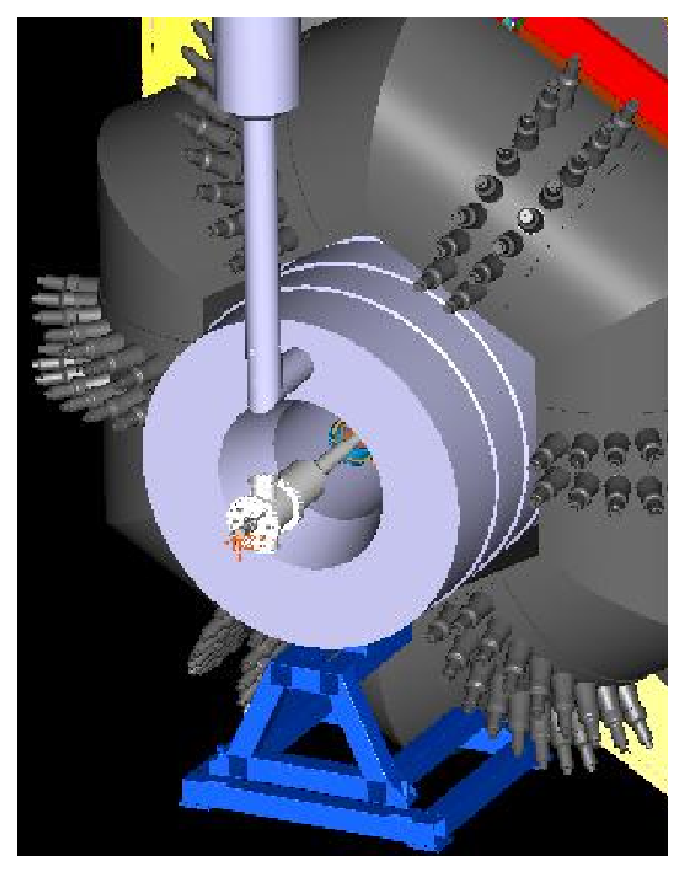
\epsfig{file=../epsfiles/target-in.eps,width=11cm}
\end{center}
\end{figure}


%\title{{\small CLAS12 DOCUMENT TO PAC30} \\
An Overview of the Hall B 12 GeV Upgrade
and the Technical Participation of the Research Groups to the Hall B 12 GeV Upgrade
}

\bigskip
\date{June 7, 2006 for JLab PAC30}
\author{ Information compiled by L.~Elouadrhiri$^{\dagger}$ for the CLAS collaboration}

\affiliation{Jefferson Lab, Newport News, VA 23606, USA}


\maketitle
\vskip 10 cm
{$^\dagger$Contact Person: latifa@jlab.org }

\newpage

\tableofcontents
\newpage
\fancypagestyle{myheading}{%                % Redefining plain style
\fancyhf{} % clear all header and footer fields
\fancyhead[C]{\vspace{0.5cm}\line(1,0){500}\vspace{-0.5cm}}
\fancyhead[l]{\mbox{\bfseries CLAS12 Technical Design Report}}
\fancyhead[r]{\mbox{\bfseries Version 1.1  \date{\today}}}
\fancyfoot[C]{\mbox{\bfseries  \thepage }}
\fancyfoot[r]{\mbox{\bfseries Drift chambers}}
\fancyfoot[l]{\vspace{-1cm}\line(1,0){500}}
}
\renewcommand{\headrulewidth}{0pt}
\renewcommand{\footrulewidth}{0pt}
\pagestyle{myheading}
\section{Tracking Requirements}


%\section{Drift Chambers Design}
\section{Drift Chamber Design}

\subsection{Overview}

The forward tracking system consists of three regions as shown in 
Fig.~\ref{fig:CLAS12 FDC} in each sector; located just before, inside, and 
just outside the torus field volume, and referred to as Regions 1, 2, and 3.  
Each chamber will have its wires arranged in two superlayers of six layers 
each, with the wires in the two superlayers strung with $\pm$6$^\circ$
stereo angles, respectively.  The cell structure will be hexagonal, that is, 
each sense wire is surrounded by six field wires.  This arrangement is 
similar to the present {\tt CLAS} design and offers good resolution with 
very good pattern recognition properties.  Refer to our article on the 
overall {\tt CLAS} detector~\cite{clasnim} and our article on the drift 
chambers themselves~\cite{dcnim} for details of the present detector and 
chambers.

%%%%%%%%%%%%%%%%%%%%%%%%%%%%%%%%%%%%%%%%%%%%%%%%%%%%%%%%%%%%%%%%%%%%%%%%
\begin{figure}[hb]
\vspace{10.6cm}
\special{psfile=umbrella.ps hscale=60 vscale=60 hoffset=60 voffset=0}
\caption{\small{Layout of the {\tt CLAS12} Forward Drift Chambers: Region~1, 
2, and 3.}}
\label{fig:CLAS12 FDC}
\end{figure}
%%%%%%%%%%%%%%%%%%%%%%%%%%%%%%%%%%%%%%%%%%%%%%%%%%%%%%%%%%%%%%%%%%%%%%%%

The major difference is that the cells cover a much smaller solid angle
than those in the present chambers, allowing efficient tracking at higher 
luminosities because the accidental occupancy from particles not associated 
with the event is smaller. Table~\ref{fwd-dc-design-parms} lists the main
design parameters for each region of the {\tt CLAS12} drift chambers.  For 
the purposes of simulating track resolutions, we assumed that the position 
resolution of the individual drift cells would be 250~$\mu$m.  For reference, 
the present {\tt CLAS} chambers have resolutions of 310, 315, and 380~$\mu$m 
for R1, R2, and R3, respectively.

%%%%%%%%%%%%%%%%%%%%%%%%%%%%%%%%%%%%%%%%%%%%%%%%%%%%%%%%%%%%%%%%%%%%%%%%%
\begin{table}[htbp]
\begin{center}
\begin{tabular} {||c|c|c|c||} \hline \hline
&{\bf Region 1}      &  {\bf Region 2} & {\bf Region 3}\\ \hline
dist. from target    & 2.1 m & 3.3 m   & 4.5 m \\ \hline
num. of superlayers  & 2 & 2   & 2 \\ \hline
layers/superlayer    & 6 & 6   & 6 \\ \hline
wires/layer          & 112 & 112   & 112 \\ \hline
cell size            & 0.75 cm & 1.18 cm   & 2.07 cm \\ \hline
active time window   & 150 ns & 250 - 500 ns & 500 ns \\ \hline
assumed resolution per wire  & 0.025 cm & 0.025 cm   & 0.025 cm \\ \hline
\end{tabular}
\caption{\small{Design parameters for the {\tt CLAS12} drift chambers.}}
\label{fwd-dc-design-parms}
\end{center}
\end{table}
%%%%%%%%%%%%%%%%%%%%%%%%%%%%%%%%%%%%%%%%%%%%%%%%%%%%%%%%%%%%%%%%%%%%%%%%%

The chambers differ from the present {\tt CLAS} chambers in a number of 
ways.  Successive superlayers have their wires arranged with a plus or 
minus 6$^{\circ}$ stereo angle; the present arrangement has an axial layer 
and a 6$^{\circ}$ stereo layer.  For the present {\tt CLAS} detector, the 
$\phi$ resolution is about four times larger than the $\theta$ resolution.  
To have more equal resolution in the two angles, we decided that we needed 
to double our effective stereo angle in order to improve the  $\phi$ 
resolution.  Unlike the present chambers, all of the wires in one of the 
superlayers are strictly parallel, and in a plane perpendicular to the wire 
direction form perfect hexagons.  This should allow a more accurate drift 
velocity calibration than the current design with its layer-to-layer 
increase in cell size.  The choice of gas; a 92:08 Argon:CO$_2$ mixture is 
a small departure from our present 90:10 mixture and should result in a 
higher and more constant drift velocity.  We plan to run with a gas gain 
of $5\cdot10^4$.

Another departure from the present design is to design every chamber (in 
all three regions) to be self-supporting in order to ensure that they are 
easy to install and remove for maintenance.  In the present {\tt CLAS}, the 
Region~1 chambers are all bound together into a single unit in order to 
maintain the wire tension without excessively thick endplates, and the 
Region~2 chambers are actually mounted onto the magnet cryostat with the 
cryostat itself maintaining the internal wire tension.  None of the present 
Region~1 or 2 chambers can be accessed individually without a lengthy 
``tension-transfer'' process.  To avoid this, we are designing the
Region~1 and Region~2 chambers to be self-supporting like our present 
Region~3 chambers.  To keep a very thin endplate (to minimize dead area), 
some of the wire tension in the Region~2 chambers will be borne by springs 
mounted to the torus cryostat; but many fewer springs than in the present 
detector.  The key to these improvements will be ultra-stiff endplate 
assemblies which obtain their stiffness by a flanged design.  

A third design change is to use 30~$\mu$m diameter sense wire rather than 
the more common 20~$\mu$m wire. Our choice of wire is 30~$\mu$m diameter, 
gold-plated tungsten for the sense wires, 140~$\mu$m diameter, gold-plated 
aluminum for the field wires and 140~$\mu$m diameter, stainless steel for
the guard wires.   This should make the chamber more robust to wire 
breakages.  Higher voltages will be required to achieve the same gas gain, 
and the resulting higher electric field in the drift cells will result in 
a more nearly constant drift velocity which should be easier to calibrate.
Prototypes are being built to study possible negative side-effects of the 
higher voltage operation such as leakage currents on the circuit boards 
and/or higher rates of cathode emission from the field wire surfaces.

Fig.~\ref{garfield} shows GARFIELD calculations for a Region~3 drift cell
with both a 20~$\mu$m and a 30~$\mu$m diameter sense wire.  Here the
cells with the thicker sense wire will have a significantly higher drift 
velocity which is desirable to reduce the time window, and hence the chamber 
occupancy.

%%%%%%%%%%%%%%%%%%%%%%%%%%%%%%%%%%%%%%%%%%%%%%%%%%%%%%%%%%%%%%%%%%%%%%%%%%%
\begin{figure}[htbp]
\vspace{12.0cm}
\special{psfile=garfield1.eps hscale=30 vscale=27 hoffset=40 voffset=165}
\special{psfile=garfield2.eps hscale=30 vscale=27 hoffset=40 voffset=-5}
\special{psfile=garfield3.eps hscale=30 vscale=27 hoffset=230 voffset=165}
\special{psfile=garfield4.eps hscale=30 vscale=27 hoffset=230 voffset=-5}
\caption{\small{GARFIELD calculations of the electric field lines (top)
and drift time vs. drift distance (bottom) for a Region~3 drift cell.  The 
left plots show the configuration with a 20~$\mu$m diameter sense wire and 
the right plots show the configuration with a 30~$\mu$m diameter sense wire.
The high voltages were set to provide the same gas gain for each
configuration.}}
\label{garfield}
\end{figure}
%%%%%%%%%%%%%%%%%%%%%%%%%%%%%%%%%%%%%%%%%%%%%%%%%%%%%%%%%%%%%%%%%%%%%%%%%%%








\subsection{Design Consideration}

\subsection{Mechanical Design}

\subsection{Alignement}

\subsection{Electrical Design}


\section{Prototyping}

\subsection{Overview}

\subsection{Design}

\subsection{Mechanical}

\subsection{Electrical}

\subsection{Results}

\section{Fabrication}

\subsection{Infrastructure}

\subsection{Toolings}

\subsection{Utilities}

\section{Assembly Installation and commissioning}

\section{Operation}

\subsection{Monitoring}

\subsection{Calibration}


\section{Expected Performances}

\subsection{Simulation}
\subsection{Reconstruction}
\subsection{Projected results}

\section{Simulation: Expected Performance}
\label{simulation}

As discussed above, the {\tt CLAS12} detector is designed to detect 
semi-inclusive and exclusive events with a modest number (up to 4 or 5) 
of outgoing hadrons.  In addition to the electron and hadrons associated 
with the event of interest, the detected event will contain both 
electromagnetic and hadronic ``accidentals''.  Because the physics goal is 
to run at beam-target luminosities of \1035 or higher, we have simulated the 
expected accidental particle flux associated with these luminosities.  Using 
a modified version of the EGS program~\cite{egs}, we simulated the total 
hadronic and electromagnetic particle fluxes generated when an electron beam 
is incident upon a liquid-hydrogen target with a luminosity of \1035.  We 
calculated the total flux through a measurement layer during its active 
(measurement) time and multiplied by the probability of the particle interacting 
in that layer and divided by the number of cells in the layer to get an estimate 
of the fractional occupancy of that layer due to background.  The expected layer 
occupancy under these conditions is on the order of 3-4\%.  Our experience with 
the present {\tt CLAS} detector is that track-finding is highly efficient if the 
accidental occupancy is less than 4\%~\cite{dcnim}.  Fig.~\ref{trkeff} shows 
the efficiency of our present tracking program for finding a track as a 
function of the fractional occupancy of Region~1, that is, the percentage of 
wires that fired for the event in question.  One can see that the efficiency
begins to fall off at a fractional occupancy of about 4\%.

%%%%%%%%%%%%%%%%%%%%%%%%%%%%%%%%%%%%%%%%%%%%%%%%%%%%%%%%%%%%%%%%%%%%%%%%%%%
\begin{figure}[htbp]
\vspace{8.0cm}
\special{psfile=trk_eff.eps hscale=90 vscale=85 hoffset=0 voffset=-280}
\caption{\small{Plot of tracking efficiency versus the fractional number
of wires with hits in Region~1 taken from Ref.~\cite{dcnim}.}}
\label{trkeff}
\end{figure}
%%%%%%%%%%%%%%%%%%%%%%%%%%%%%%%%%%%%%%%%%%%%%%%%%%%%%%%%%%%%%%%%%%%%%%%%%%%

\subsection{Rate Dependence of the Tracking Efficiency}

We use two methods to simulate our rate-dependent efficiency:

\begin{enumerate}
\item we use a GEANT3 or GEANT4 based simulation to estimate the number
of wires with hits in Region~1 during its estimated active time window
of 150~ns.  We then infer the tracking efficiency from Fig.~\ref{trkeff}.

\item we use a GEANT3-based model of the tracking chambers, magnetic
field and key absorbers to simulate background during an event.  We
combine this background event with a simulated single-particle track
through the chambers, and run our normal track reconstruction code on
the combined event.
\end{enumerate}

Our GEANT3 rate simulations indicate that the number of accidental tracks
(not associated with the event in question) crossing the Reg. 1
drift chambers during their sensitive time at a luminosity of \1035
is signicantly less than that simulated for a recent experiment:
E1DVCS which employed a similar solenoidal shield for Moller electrons
and which ran at a luminosity of $2\cdot 10^{34}$~cm$^{-2}$s$^{-1}$.
We are continuing to run more detailed simulations to verify this
result.

\subsection{Charged Track Resolution}

We have also used two methods to simulate resolutions.  In one, we use the 
MOMRES~\cite{momres} program to estimate the position, angle, and momentum 
resolution in the bend plane and a simple linear fit to estimate the position 
and angular resolution out of the bend plane.  The second method is to use 
the full power of a GEANT3 simulation and a full track reconstruction to 
estimate the resolution on the five track parameters simultaneously.

We studied the position, angle, and momentum resolution for a number of 
possible detector options using MOMRES.  The input file to MOMRES
characterized the detector position, material thickness, and estimated hit 
resolution for a particular track angle.  We also produced a $B$-field file 
that was a tabulation of the $B$-field strength vs. path length for a 
particular track angle.  These, and the desired range of momenta, were then
used to calculate the expected components of the resolutions due to multiple 
scattering and measurement resolution.  We fit these outputs to the expected 
kinematic form.  From these fits we extracted two parameters ($\sigma$1 and 
$\sigma$2) for each of the three terms ($dp/p$, $d\theta$, $dx$).  These six 
parameters summarize the output of MOMRES.  In addition, we calculated the 
angle resolution in the non-bend plane in a manner analogous to that of MOMRES, 
using estimates for the effects of multiple scattering and measurement error, 
fitting the resulting smeared trajectory by a straight line, and extracting 
the $\sigma$1 and $\sigma$2 parameters that characterize the resolution in 
this non-bend plane angle.  Thus, eight parameters for each value of track 
angle fully characterize the tracking resolution for any one detector option.  
Fig.~\ref{dpvstheta} shows the momentum resolutions for tracks emitted at 
various angles.

%%%%%%%%%%%%%%%%%%%%%% Figure : dp/p vs. theta %%%%%%%%%%%%%%%%%%%%
\begin{figure}[ht]
\vspace{9.0cm}
\special{psfile=dpvstheta.ps hscale=60 vscale=45 hoffset=50 voffset=255 angle=-90}
\caption{\small{Resolution simulated using MOMRES plotted vs. particle 
momentum for tracks emitted at various angles.  The momentum resolution
is better at small angles because the traversed integral $B$-field is
higher.}}
\label{dpvstheta}
\end{figure}
%%%%%%%%%%%%%%%%%%%%%%%%%%%%%%%%%%%%%%%%%%%%%%%%%%%%%%%%%%%%%%%%%%%%%%%%%

Looking at Fig.~\ref{comparep} we see three graphs of the 
momentum resolution plotted versus momentum.  One is for a MOMRES 
calculation of our standard set-up, with 6 layers of a Forward Silicon Tracker
(FSVT) followed by our three regions of drift chamber; a second is for the 
same setup but without the FSVT.  Finally, a third curve 
shows the result of increasing the spatial resolution of the drift chambers 
from 250 to 350~$\mu$.  Note that our standard case, with the FSVT, has better 
resolution at high momentum because of the extra measurement points from the
FSVT, but has worse resolution at low momenta, because of the additional
multiple scattering of six planes of FSVT.  Fig.~\ref{compareth} shows the 
three cases again; there is not much difference between them.  Finally, 
Figs.~\ref{comparex} shows the dramatic improvement in vertex resolution 
provided by the FSVT. 

%%%%%%%%%%%%%%%%%%%%%% Figure : dp/p: 4 cases %%%%%%%%%%%%%%%%%%%%
\begin{figure}[htpb]
\vspace{9.0cm}
\special{psfile=comp_p_paper.eps hscale=55 vscale=45 hoffset=70 voffset=0}
\caption{\small{Momentum resolution simulated using MOMRES (for 3 cases)
plotted vs. particle momentum for tracks emitted at 15$^\circ$.}}
\label{comparep}
\end{figure}
%%%%%%%%%%%%%%%%%%%%%%%%%%%%%%%%%%%%%%%%%%%%%%%%%%%%%%%%%%%%%%%%%%%%%%%%%

%%%%%%%%%%%%%%%%%%%%%% Figure : dt 4 cases %%%%%%%%%%%%%%%%%%%%%%%%%%%%%%
\begin{figure}[htpb]
\vspace{9.0cm}
\special{psfile=comp_th_paper.eps hscale=55 vscale=45 hoffset=70 voffset=0}
\caption{\small{Theta resolution simulated using MOMRES (for 3 cases)
plotted vs. particle momentum for tracks emitted at 15$^\circ$. }}
\label{compareth}
\end{figure}
%%%%%%%%%%%%%%%%%%%%%%%%%%%%%%%%%%%%%%%%%%%%%%%%%%%%%%%%%%%%%%%%%%%%%%%%%

%%%%%%%%%%%%%%%%%%%%%% Figure : dx 4 cases %%%%%%%%%%%%%%%%%%%%%%%%%%%%%%
\begin{figure}[htpb]
\vspace{9.0cm}
\special{psfile=comp_x_paper.eps hscale=55 vscale=45 hoffset=70 voffset=0}
\caption{\small{Impact parameter resolution simulated using MOMRES (for 3 cases)
plotted vs. particle momentum for tracks emitted at 15$^\circ$.}}
\label{comparex}
\end{figure}
%%%%%%%%%%%%%%%%%%%%%%%%%%%%%%%%%%%%%%%%%%%%%%%%%%%%%%%%%%%%%%%%%%%%%%%%%

Fig.~\ref{resol} provides a few more results of these studies to
parameterize and understand the resolution expected for the {\tt CLAS12}
tracking system.  The plots show the expected angular resolution, the 
expected position resolution, and the expected momentum resolution
for different angle bins, each as a function of momentum.  These plots
were made using the current design of the tracking system.

%%%%%%%%%%%%%%%%%%%%%%%%%%%%%%%%%%%%%%%%%%%%%%%%%%%%%%%%%%%%%%%%%%%%%%%%%
\begin{figure}[htbp]
\vspace{12.0cm}
\special{psfile=resol_1.eps hscale=35 vscale=30 hoffset=15 voffset=160}
\special{psfile=resol_2.eps hscale=35 vscale=30 hoffset=225 voffset=160}
\special{psfile=resol_3.eps hscale=35 vscale=30 hoffset=115 voffset=-10}
\caption{\small{Simulation results for the {\tt CLAS12} tracking system
showing the expected angular resolution, position resolution, and
momentum resolution for different angle bins as a function of momentum.}
\label{resol}}
\end{figure}
%%%%%%%%%%%%%%%%%%%%%%%%%%%%%%%%%%%%%%%%%%%%%%%%%%%%%%%%%%%%%%%%%%%%%%%%%


\section{Expected Physics Performance}

We used a series of programs to calculate the acceptance and reconstructed 
physics parameters for event types of interest.  The program {\it clasev}
\cite{clasev} served as an event generator and analysis program. 
Depending on the value of input flags, it generates certain types of 
events; that is, it produces a set of 4-momenta for the primary hadrons 
in the hadronic center-of-mass and allows some of them to decay into the 
final-state hadrons and transforms their momenta to the lab system.  For 
each final-state track, it calls {\tt FASTMC} to determine if the track 
falls within a fiducial acceptance window and to determine its final, 
smeared lab momentum.  It then produces selected physics analysis variables 
such as missing mass from calculations involving the smeared momenta of 
those tracks that were accepted. 

Fig.~\ref{massplot} shows the expected missing mass resolution 
expected for {\tt CLAS12} from simulation studies based on the current
design specifications for a number of different reactions.  For all
cases studied the results are quite encouraging in terms of identifying
the missing particle cleanly for each reaction.

%%%%%%%%%%%%%%%%%%%%%%%%%%%%%%%%%%%%%%%%%%%%%%%%%%%%%%%%%%%%%%%%%%%%%%%%%%%
\begin{figure}[htbp]
\vspace{14.0cm}
\special{psfile=mm1.ps hscale=39 vscale=36 hoffset=-10 voffset=160}
\special{psfile=mm2.ps hscale=39 vscale=36 hoffset=225 voffset=160}
\special{psfile=mm3.ps hscale=40 vscale=37 hoffset=-10 voffset=-55}
\special{psfile=mm4.ps hscale=40 vscale=37 hoffset=230 voffset=-55}
\caption{\small{Simulation results highlighting the expected missing
mass resolution of {\tt CLAS12} with the nominal design specifications for
the drift chambers.  Shown are the spectra for the reactions
$ep \to e'\pi+X$ (UL), $ep \to e'K^+X$ (UR), $ep \to e'p\pi^+X$ (LL),
and $ep \to e\rho^+X$ (LR).}}
\label{massplot}
\end{figure}
%%%%%%%%%%%%%%%%%%%%%%%%%%%%%%%%%%%%%%%%%%%%%%%%%%%%%%%%%%%%%%%%%%%%%%%%%%%

\section{Cost and Schedule}

\section{Responsibilities}


\newpage

\appendix
\section{Previous Experience with CLAS Drift Chambers}




%\input{experiment-final.tex}
\end{document}
